\documentclass[11pt,a4paper]{article}
\usepackage[T1]{fontenc}
\usepackage[utf8]{inputenc}
\usepackage{lmodern,microtype}
\usepackage[margin=26mm,headheight=14pt]{geometry}
\usepackage{amsmath,amssymb,amsthm,mathtools}
\usepackage{booktabs,array}
\usepackage{tikz}
\usepackage{xcolor}
\usepackage{enumitem}
\usepackage{listings}
\usepackage{fancyhdr}
\usepackage[hidelinks]{hyperref}
\usepackage{bookmark}
\hypersetup{pdftitle={Record bonds and a mesh-pattern generating function: a proof for OEIS A289587},pdfauthor={OpenAI},pdfsubject={Combinatorial proof, refined enumeration, exact algorithms and asymptotics}}
\newtheorem{theorem}{Theorem}[section]
\newtheorem{lemma}[theorem]{Lemma}
\newtheorem{proposition}[theorem]{Proposition}
\newtheorem{corollary}[theorem]{Corollary}
\theoremstyle{definition}
\newtheorem{definition}[theorem]{Definition}
\newtheorem{example}[theorem]{Example}
\theoremstyle{remark}
\newtheorem{remark}[theorem]{Remark}
\newcommand{\Av}{\operatorname{Av}}
\newcommand{\rec}{\operatorname{rec}}
\newcommand{\Cat}{\mathrm{Cat}}
\newcommand{\ind}{\mathbf{1}}
\newcommand{\Rone}{\mathcal{R}_{174}}
\newcommand{\Rtwo}{\mathcal{R}_{234}}
\newcommand{\class}{\mathcal{A}}
\newcommand{\core}{\mathcal{R}}
\DeclareMathOperator{\Seq}{Seq}
\setlist{nosep}
\setcounter{tocdepth}{1}
\setlength{\parskip}{3pt}
\setlength{\emergencystretch}{2em}
\pagestyle{fancy}
\fancyhf{}
\fancyhead[L]{\small Record bonds and mesh-pattern avoidance}
\fancyhead[R]{\small OEIS A289587}
\fancyfoot[C]{\thepage}
\renewcommand{\headrulewidth}{0.3pt}
\lstset{basicstyle=\small\ttfamily,columns=fullflexible,keepspaces=true,
  frame=single,framerule=0.3pt,breaklines=true,showstringspaces=false,
  aboveskip=10pt,belowskip=10pt}
\title{\textbf{Record bonds and a mesh-pattern\newline generating function}\\[5pt]
\large A proof of the conjecture for OEIS A289587}
\author{}
\date{September 20, 2026}

\begin{document}
\maketitle
\vspace{-1.5em}
\begin{abstract}
We prove the conjectured ordinary generating function for the number of
permutations avoiding the classical pattern $321$ and either of the two
mesh patterns designated $(12,174)$ and $(12,234)$. The crucial step is a
structural characterization: in the first class, the mesh restriction is
exactly the conjunction of having no adjacent consecutive ascent beginning
at a left-to-right maximum and having at most one singleton direct-sum
component. A canonical contraction of record runs reduces the enumeration
to the Narayana refinement of $321$-avoiding permutations. This gives the
conjectured algebraic generating function, a refinement by three statistics,
positive coefficient recurrences, an algorithm using linearly many integer
arithmetic operations, and a two-term asymptotic expansion. The proof is
self-contained at the enumerative level. Reproducible exhaustive and exact
computations accompany the article.
\end{abstract}
\tableofcontents
\newpage

\section{The problem and the result}

Let $a_n$ be the number of length-$n$ permutations avoiding $321$ and the
mesh pattern $(12,174)$. We include the empty permutation, so $a_0=1$.
OEIS A289587 identifies the same sequence with avoidance of $(12,234)$ and
attributes the following generating-function conjecture to Thomas Scheuerle,
December 23, 2025 \cite{oeis}. The mesh-label convention is explained in
Christian Sievers's December 2025 SeqFan discussion \cite{seqfan}; we specify
the actual shaded sets below, so no encoding convention is left implicit.

Write
\begin{align}
 D(x)&=x^4-2x^3-5x^2-2x+1,\label{eq:D}\\
 P(x)&=x^4+4x^3+11x^2+10x+3,\label{eq:P}\\
 Q(x)&=x^2+5x+3.\label{eq:Q}
\end{align}

\begin{theorem}[The conjectured generating function]\label{thm:main}
For every $n\geq 0$, the two mesh-avoidance classes in A289587 are equinumerous.
Their common ordinary generating function is
\begin{equation}\label{eq:main}
 \boxed{\displaystyle
 A(x)=\sum_{n\geq0}a_nx^n
 =\frac{P(x)-Q(x)\sqrt{D(x)}}{8x(1+x)^2}.}
\end{equation}
Here $\sqrt{D(x)}$ means the formal power-series square root with constant
term $1$. The apparent singularity at $x=0$ is removable.
\end{theorem}

The first terms are
\[
1,1,1,3,6,18,47,139,405,1225,3740,11602,36357,115049,\ldots.
\]
The interesting issue is not recognizing a square root from these numbers.
A mesh condition quantifies over two selected entries and the emptiness of
several surrounding rectangles. It can detect distant entries and therefore
need not be reducible to a local prohibition. In the present case there is
indeed an additional global obstruction: two singleton direct-sum components,
even when separated by a nontrivial component. The proof isolates this
obstruction before performing any generating-function manipulation.

The ambient class $\Av(321)$ belongs to the central Catalan family of
permutation enumeration. We derive the required Catalan--Narayana
correspondence explicitly rather than using an unexplained formula for
indecomposable permutations. The substantive new argument within this note
is the mesh characterization and its connection to canonical record-run
contraction.

\paragraph{Status and scope.}
The OEIS entry consulted on September 20, 2026 still explicitly labels
\eqref{eq:main} conjectural. This article supplies an independent proof of
that formula; it does not assert an exhaustive bibliographic priority search.
The two-pattern equivalence will also be proved, not inferred from agreement
of initial terms.

\section{Mesh patterns, records, and direct sums}

\subsection{The two shaded patterns}

For a permutation $\pi=\pi_1\cdots\pi_n$, a classical $321$ occurrence is a
triple $i<j<k$ with $\pi_i>\pi_j>\pi_k$. A $12$ occurrence is a pair
$i<j$ with $a=\pi_i<b=\pi_j$.

Relative to the latter pair, every other point $(k,\pi_k)$ belongs to one
of nine open rectangles. Its first cell coordinate $I\in\{0,1,2\}$ records
whether $k$ is before $i$, between $i$ and $j$, or after $j$; its second
coordinate $J$ records whether $\pi_k$ is below $a$, between $a$ and $b$,
or above $b$. A mesh occurrence requires the rectangles in a specified set
to be empty. This is the usual mesh-pattern framework
\cite{branden-claesson}, specialized here to a length-two pattern.

For the two labels in question, the shaded sets are
\begin{align}
 \Rone&=\{(0,1),(0,2),(1,0),(1,2),(2,1)\},\label{eq:174}\\
 \Rtwo&=\{(0,1),(1,0),(1,2),(2,0),(2,1)\}.\label{eq:234}
\end{align}
The convention in \cite{seqfan} assigns cell $(I,J)$ the weight
$2^{3I+J}$; summing the weights gives the displayed labels. These labels
only name the patterns and play no arithmetic role in the proof.

\begin{figure}[ht]
\centering
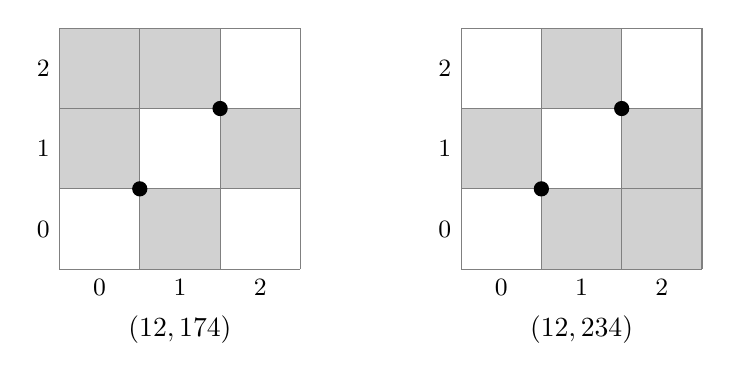
\begin{tikzpicture}[scale=1.02]
 \begin{scope}
  \foreach \i/\j in {0/1,0/2,1/0,1/2,2/1}
   \fill[black!18] (\i,\j) rectangle +(1,1);
  \draw[step=1,black!50,thin] (0,0) grid (3,3);
  \fill (1,1) circle (2.7pt); \fill (2,2) circle (2.7pt);
  \foreach \i in {0,1,2} \node[below] at (\i+.5,0) {\small $\i$};
  \foreach \j in {0,1,2} \node[left] at (0,\j+.5) {\small $\j$};
  \node at (1.5,-.75) {$(12,174)$};
 \end{scope}
 \begin{scope}[xshift=5cm]
  \foreach \i/\j in {0/1,1/0,1/2,2/0,2/1}
   \fill[black!18] (\i,\j) rectangle +(1,1);
  \draw[step=1,black!50,thin] (0,0) grid (3,3);
  \fill (1,1) circle (2.7pt); \fill (2,2) circle (2.7pt);
  \foreach \i in {0,1,2} \node[below] at (\i+.5,0) {\small $\i$};
  \foreach \j in {0,1,2} \node[left] at (0,\j+.5) {\small $\j$};
  \node at (1.5,-.75) {$(12,234)$};
 \end{scope}
\end{tikzpicture}
\caption{Gray cells must contain no other permutation points. Reflecting
across the diagonal exchanges the two shaded sets. Outer cells represent
unbounded rectangles, drawn here at finite size.}
\label{fig:mesh}
\end{figure}

\begin{lemma}[Inverse equivalence]\label{lem:inverse}
The map $\pi\mapsto\pi^{-1}$ is a bijection between the two classes counted
in Theorem~\ref{thm:main}.
\end{lemma}
\begin{proof}
Inverting a permutation transposes its point plot. The increasing pattern
$12$ is invariant under transposition, and transposition of every cell in
\eqref{eq:174} gives exactly \eqref{eq:234}. The classical pattern $321$
is also its own inverse. Thus inversion preserves $321$-avoidance and
exchanges the two mesh restrictions, in both directions.
\end{proof}

We henceforth work with $(12,174)$. Refinements by records below refer to
this class; the inverse bijection need not preserve the record statistic.

\subsection{The structural statistics}

An entry $\pi_i$ is a \emph{record}, or left-to-right maximum, when
$\pi_h<\pi_i$ for every $h<i$. Write $\rec(\pi)$ for the number of records.

\begin{definition}
An \emph{upper bond} is an index $i<n$ such that $\pi_i$ is a record and
$\pi_{i+1}=\pi_i+1$. A maximal chain of upper bonds is called a
\emph{record run}. A record not in any upper bond is a record run of length
one.
\end{definition}

The qualifier ``upper'' is important: we do not forbid every adjacent
consecutive ascent. The ascent must start at a record.

For $\alpha\in S_p$ and $\beta\in S_q$, their direct sum is
\[
 \alpha\oplus\beta
 =\alpha_1\cdots\alpha_p\,(p+\beta_1)\cdots(p+\beta_q).
\]
A permutation is \emph{sum-indecomposable} if it is nonempty and has no
nontrivial such decomposition. A \emph{sum cut} at $t$ is characterized by
\[
 \{\pi_1,\ldots,\pi_t\}=\{1,\ldots,t\}.
\]
Cutting at every sum cut gives the unique sequence of sum-indecomposable
components. A singleton component means a component equal to the
one-entry permutation $1$. Equivalently, a point at position $i$ is such a
component when $\pi_i=i$ and the cuts immediately before and after that
point are sum cuts. Boundary cuts at $0$ and $n$ are allowed.

\section{The structural characterization}

\begin{theorem}[Local bonds and a global obstruction]\label{thm:structure}
A $321$-avoiding permutation contains $(12,174)$ if and only if it has an
upper bond or at least two singleton direct-sum components.
Consequently, it avoids $(12,174)$ exactly when neither obstruction occurs.
\end{theorem}

\begin{proof}
Suppose first that positions $i<j$, with values $a=\pi_i<b=\pi_j$, form
an occurrence of $(12,174)$. The shaded rectangles say the following:
all entries before $i$ are less than $a$; all entries strictly between
$i$ and $j$ have values strictly between $a$ and $b$; and every value
strictly between $a$ and $b$ occurs between $i$ and $j$. The last assertion
uses both the forbidden middle-valued prefix and the forbidden middle-valued
suffix.

It follows that the position interval $[i,j]$ contains exactly the value
interval $[a,b]$, with the endpoints fixed at $a$ and $b$. In particular,
\begin{equation}\label{eq:interval-count}
 j-i=b-a,\qquad a\geq i.
\end{equation}
There are two different cases.

\emph{Case $a>i$.} There are $a-1$ values below $a$, but the prefix before
$i$ contains only $i-1$ of them, and the block from $i$ to $j$ contains none.
Therefore a value $c<a$ occurs after $j$. If the block from $i$ to $j$
had a descent $\pi_u>\pi_v$ with $u<v$, then
$\pi_u>\pi_v>c$, at positions $u<v<\pi^{-1}(c)$, would form $321$.
The block is therefore increasing. Since its values are exactly
$a,a+1,\ldots,b$, its first two entries are $a,a+1$. The first is a record,
so this is an upper bond.

\emph{Case $a=i$.} The prefix before $i$ is precisely the set
$\{1,\ldots,i-1\}$. Equation~\eqref{eq:interval-count} gives $j=b$.
The initial $j$ positions contain exactly $\{1,\ldots,j\}$, and their
last entry is $j$. Thus there are sum cuts at $i-1,i,j-1,j$, with repeated
cuts identified when $j=i+1$. The entries at $i$ and $j$ are two distinct
singleton components. Notice that the middle block need not be increasing
in this case.

Conversely, an upper bond $a,a+1$ occupies adjacent positions. There are
neither intermediate positions nor intermediate values, and every earlier
entry is below $a$ by the record condition. All five required rectangles
are empty, so the bond is a mesh occurrence.

Finally, suppose there are two singleton components at positions $i<j$.
Their values are $i$ and $j$. Entries before $i$ are below $i$, entries
between the two components have values between $i$ and $j$, and entries
after $j$ are above $j$. The selected singleton entries therefore form an
occurrence of $(12,174)$. This proves both implications.
\end{proof}

\begin{example}[Why both obstructions matter]
The permutation $231$ is excluded because $2,3$ is an upper bond.
The permutation $1324=1\oplus21\oplus1$ has no upper bond, but its two
singleton components form a mesh occurrence. On the other hand, $4123$
is allowed: its consecutive ascents $1,2$ and $2,3$ are not record ascents,
and it is sum-indecomposable. Thus neither ordinary succession avoidance
nor merely banning adjacent singleton components gives the right class.
\end{example}

\begin{lemma}[Bonds at component boundaries]\label{lem:boundary}
An upper bond crossing a direct-sum boundary consists of two adjacent
singleton components. Within a component, being a record is equivalent
to being a record after standardizing that component.
\end{lemma}
\begin{proof}
At a sum cut $i$, the largest value in the first $i$ positions is $i$.
If $\pi_i$ is a record then $\pi_i=i$; if the next entry is consecutive,
then $\pi_{i+1}=i+1$. This forces additional sum cuts at $i-1$ and $i+1$,
so both entries are singleton components. For the second assertion,
all preceding components contain values smaller than every value of the
current component.
\end{proof}

Let $\core$ be the class of nontrivial (size at least two)
sum-indecomposable $321$-avoiding permutations with no upper bonds, and put
\begin{equation}\label{eq:Rdef}
 R(x)=\sum_{\pi\in\core}x^{|\pi|}.
\end{equation}
The characterization and the boundary lemma give a unique decomposition of
an allowed permutation: either a sequence of $\core$-components, or a
sequence of such components followed by one singleton and another sequence
of such components. Therefore
\begin{equation}\label{eq:assembly}
 \boxed{\displaystyle A(x)=\frac{1}{1-R(x)}+
                          \frac{x}{(1-R(x))^2}.}
\end{equation}
The second term counts an actual singleton component, not a marked arbitrary
position. With $m$ nontrivial components there are exactly $m+1$ possible
locations for it. Because $R(0)=0$, these geometric-series constructions
are legitimate formal power series.

\section{Records in the Catalan class}

To determine $R$, we first count all $321$-avoiding permutations by records.
Define
\[
 C(x,y)=\sum_{\pi\in\Av(321)}x^{|\pi|}y^{\rec(\pi)},
\]
including the empty permutation with weight $1$.

\subsection{An explicit Dyck-path correspondence}

\begin{lemma}\label{lem:nonrecords}
In a $321$-avoiding permutation, the subsequence of nonrecords is increasing.
Conversely, a permutation whose nonrecords form an increasing subsequence
avoids $321$.
\end{lemma}
\begin{proof}
If nonrecords $\pi_j>\pi_k$ occur at $j<k$, the fact that $\pi_j$ is not a
record supplies an earlier $\pi_i>\pi_j$, producing $321$. Conversely,
records themselves are increasing. If both records and nonrecords are
increasing subsequences, any three entries contain two from the same
subsequence, so they cannot be decreasing.
\end{proof}

For a nonempty $321$-avoider, list its record positions and values as
\[
 1=p_1<p_2<\cdots<p_k,\qquad
 v_1<v_2<\cdots<v_k=n.
\]
Set $v_0=0$ and $p_{k+1}=n+1$. Associate the path
\begin{equation}\label{eq:dyck-map}
 U^{v_1-v_0}D^{p_2-p_1}
 U^{v_2-v_1}D^{p_3-p_2}\cdots
 U^{v_k-v_{k-1}}D^{p_{k+1}-p_k},
\end{equation}
where $U=(1,1)$ and $D=(1,-1)$.
The path has $n$ steps of each kind, positive run lengths, and $k$ peaks.
Before the next record at $p_{j+1}$, the permutation has used
$p_{j+1}-1$ different values not exceeding $v_j$. Hence
\begin{equation}\label{eq:dyck-inequality}
 v_j\geq p_{j+1}-1.
\end{equation}
This is exactly the assertion that the path remains nonnegative at the end
of its $j$th descent run, and therefore everywhere.

Conversely, read the cumulative ascent lengths and descent lengths from a
Dyck path. They recover the $v_j$ and $p_j$ in \eqref{eq:dyck-map}.
Place the prescribed record values in their prescribed positions and fill
all other positions increasingly with the remaining values. Inequality
\eqref{eq:dyck-inequality} guarantees enough unused values below $v_j$ to
fill every nonrecord position before $p_{j+1}$. Thus these fillings really
are nonrecords, while each designated record exceeds all preceding values.
Lemma~\ref{lem:nonrecords} proves $321$-avoidance. This is an inverse
construction, establishing a bijection in which records correspond to peaks.

\subsection{The functional equation and Narayana numbers}

A nonempty Dyck path has its unique first-return form $U\,H\,D\,K$.
When $H$ is empty, the initial $UD$ contributes one peak; otherwise the
peaks are exactly those in $H$ and $K$. Marking semilength by $x$ and
peaks by $y$ gives
\begin{equation}\label{eq:C}
 C=1+xyC+x(C-1)C
   =1+xC(C+y-1).
\end{equation}
In particular $C(x,1)=1+xC(x,1)^2$, the Catalan generating function.

If $W=C-1$, then $W=x(W+1)(W+y)$. Lagrange inversion gives, for $n\geq1$,
\begin{align}
 [x^ny^k]C
 &=\frac1n[t^{n-1}y^k](t+1)^n(t+y)^n\notag\\
 &=\frac1n\binom nk\binom n{k-1}
 =:N(n,k).\label{eq:Narayana}
\end{align}
We set $N(n,k)=0$ outside $n\geq1$, $1\leq k\leq n$.
These are the Narayana numbers; the derivation also establishes the precise
record statistic being used. Standard formal inversion and later analytic
transfer may be found in \cite{flajolet-sedgewick}.

\subsection{Removing the direct-sum decomposition}

Let $I(x,y)$ count nontrivial sum-indecomposable $321$-avoiders by size and
records. Direct sum preserves $321$-avoidance, and records are additive
under direct sum. Each indecomposable component is either a singleton of
weight $xy$ or an object counted by $I$. Therefore
\[
 C=\frac{1}{1-xy-I}.
\]
Combining this with \eqref{eq:C} yields the useful identity
\begin{equation}\label{eq:I}
 I=1-\frac1C-xy=x(C-1).
\end{equation}
In particular $[x^ny^k]I=N(n-1,k)$ for $n\geq2$. Substituting $I=xW$
into the equation for $W$ gives
\begin{equation}\label{eq:Iquad}
 I^2+\bigl(x(1+y)-1\bigr)I+x^2y=0.
\end{equation}
The desired solution is the one with zero constant term.

\section{Canonical contraction of record runs}

We now refine \eqref{eq:Rdef} by records:
\begin{equation}\label{eq:Rxy}
 R(x,y)=\sum_{\pi\in\core}x^{|\pi|}y^{\rec(\pi)},
 \qquad R(x)=R(x,1).
\end{equation}

\begin{theorem}[Record-run contraction]\label{thm:contraction}
Every nontrivial sum-indecomposable $321$-avoiding permutation is uniquely
obtained from a member of $\core$ by replacing each record with a nonempty
increasing interval of consecutive values. Nonrecord entries remain single.
All record-run lengths may be chosen independently.
\end{theorem}

\begin{proof}
Start with such an indecomposable permutation $\pi$. Partition its records
into maximal record runs, each occupying consecutive positions and carrying
consecutive increasing values. Treat each nonrecord as a one-point block.
Every block is therefore both a position interval and a value interval.
Contract the blocks and standardize their values to obtain a permutation
$\sigma$.

\emph{Avoidance and record status.} Selecting one representative from each
block gives $\sigma$ as a classical pattern of $\pi$, so it avoids $321$.
The value intervals of different blocks are disjoint and totally ordered.
A block is a record block exactly when all preceding blocks have smaller
value intervals. A nonrecord's earlier larger witness lies in a different
block and survives contraction. Thus records and nonrecords are preserved
at the block level.

\emph{No new upper bond.} Suppose two adjacent entries of $\sigma$ formed
an upper bond. Both entries would be records. Their original blocks are
adjacent in position, and consecutive block ranks mean that no value block
lies between their value intervals. Those intervals must therefore be
consecutive as integer intervals. Their concatenation is a longer increasing
record run in $\pi$, contradicting maximality. So $\sigma$ has no upper bond.

\emph{Indecomposability of the contraction.} A sum cut between contracted
blocks would lift to the corresponding cut in $\pi$, since each block is
an entire value interval. Thus $\sigma$ is indecomposable. It cannot have
size one: a one-block original permutation would be increasing, hence
decomposable if its size exceeded one. Therefore $\sigma\in\core$.

Conversely, take $\sigma\in\core$ and replace each record by an arbitrary
nonempty increasing interval block, leaving nonrecords as singleton blocks.
The relative order of all blocks is prescribed by $\sigma$. A decreasing
triple cannot use two points of an increasing block; if it uses three
blocks it projects to a $321$ in $\sigma$. Hence avoidance is preserved.
The same block-order observation shows that every inflated record consists
entirely of records, while an inflated nonrecord remains a nonrecord.

A hypothetical sum cut in the inflated permutation either lies between
blocks or inside a block. In the former case it descends to a sum cut of
$\sigma$. In the latter case, all earlier blocks must have smaller values
than that block and all later blocks must have larger values. The underlying
entry would then be a singleton direct-sum component of $\sigma$, also
impossible in a nontrivial indecomposable permutation. Thus inflation
preserves indecomposability.

Every bond internal to an inflated record block is an upper bond. No upper
bond crosses two blocks: otherwise their underlying entries would already
be adjacent consecutive records in $\sigma$. Consequently the inflated
blocks are exactly the maximal record runs, together with the unchanged
nonrecords. Contracting recovers $\sigma$ and all chosen lengths. This proves
existence, uniqueness, and the inverse property.
\end{proof}

\begin{example}
The indecomposable permutation $235614$ contracts to $2413$. The record
blocks are $23$ and $56$, while $1$ and $4$ are unchanged nonrecords.
The core has block lengths $(2,2,1,1)$; inflating its two records by those
lengths reconstructs $235614$. In contrast, the consecutive lower run
$123$ in $4123$ is not contracted.
\end{example}

A record of weight $xy$ becomes a nonempty record run of weight
\[
 xy+(xy)^2+(xy)^3+\cdots=\frac{xy}{1-xy}.
\]
Theorem~\ref{thm:contraction} therefore translates to
\begin{equation}\label{eq:inflateGF}
 I(x,y)=R\!\left(x,\frac{y}{1-xy}\right).
\end{equation}
The inverse formal substitution is $y\mapsto y/(1+xy)$, giving
\begin{equation}\label{eq:deflateGF}
 \boxed{\displaystyle R(x,y)=I\!\left(x,\frac{y}{1+xy}\right).}
\end{equation}
These substitutions are well-defined coefficientwise in $x$: all
coefficients are polynomials in $y$, and the substituted series have
invertible denominators with constant term $1$. The alternating signs in
the inverse substitution express an inversion of a proved bijection, not
an unmotivated guess or an assumed inclusion--exclusion rule.

\section{Derivation of the conjectured expression}

Substitute \eqref{eq:deflateGF} into \eqref{eq:Iquad} and clear the
invertible denominator $1+xy$. We obtain
\begin{equation}\label{eq:Rquad-biv}
 (1+xy)R(x,y)^2+(x+x^2y-1)R(x,y)+x^2y=0.
\end{equation}
Setting $y=1$ gives
\begin{equation}\label{eq:Rquad}
 \boxed{(1+x)R^2+(x+x^2-1)R+x^2=0.}
\end{equation}
Equivalently,
\begin{equation}\label{eq:Rpositive}
 R=x^2+(x+x^2)R+(1+x)R^2.
\end{equation}
This determines $R$ uniquely from its zero constant term; coefficient
recursion also gives $[x]R=0$.

The discriminant of \eqref{eq:Rquad} is
\[
 (1-x-x^2)^2-4x^2(1+x)=D(x).
\]
The correct root is therefore
\begin{equation}\label{eq:Rroot}
 R(x)=\frac{1-x-x^2-\sqrt{D(x)}}{2(1+x)}.
\end{equation}
The other root has constant term $1$ and cannot count a class whose members
have size at least two. The first core coefficients are
\[
 R=x^2+x^3+3x^4+7x^5+19x^6+53x^7+153x^8+453x^9
       +1367x^{10}+4191x^{11}+\cdots.
\]

Substituting \eqref{eq:Rroot} into the combinatorial assembly formula
\eqref{eq:assembly} and simplifying gives \eqref{eq:main}. For clarity,
the following polynomial certificates make this last algebraic step
checkable without trusting symbolic simplification. Put
\[
 G(x,r)=(1+x)r^2+(x+x^2-1)r+x^2,
 \qquad s=1-x-x^2-2(1+x)r.
\]
Then direct expansion gives
\begin{align}
 s^2-D(x)&=4(1+x)G(x,r),\label{eq:cert1}\\
 (P-Qs)(1-r)^2-8x(1+x)^2(1-r+x)
 &=2\bigl(Qr-3x^2-7x-3\bigr)G(x,r).\label{eq:cert2}
\end{align}
At $r=R(x)$, the right sides vanish, and $s$ has constant term $1$.
Thus $s=\sqrt{D(x)}$ and \eqref{eq:cert2} proves the desired identity
with \eqref{eq:assembly}. This completes the proof of
Theorem~\ref{thm:main}.

An additional compact algebraic certificate is
\begin{equation}\label{eq:Aquad}
 4x(1+x)^2 A(x)^2-P(x)A(x)+2x^3+8x^2+9x+3=0,
 \qquad A(0)=1.
\end{equation}
The constant term condition and the nonzero coefficient $-P(0)=-3$
determine a unique formal solution. This identity follows either from
\eqref{eq:main} by squaring or from the two preceding polynomial
certificates.

\section{Refinements and explicit core coefficients}

\subsection{Records, nontrivial components, and the singleton}

For $\pi\in\class$, let $m(\pi)$ count its nontrivial direct-sum components,
and let $s(\pi)\in\{0,1\}$ count its singleton components. The same unique
decomposition used earlier gives the full refinement
\begin{equation}\label{eq:refinedA}
 \boxed{\displaystyle
 \sum_{\pi\in\class}x^{|\pi|}y^{\rec(\pi)}u^{m(\pi)}v^{s(\pi)}
 =\frac{1}{1-uR(x,y)}+
   \frac{vxy}{(1-uR(x,y))^2}.}
\end{equation}
Thus permutations with $m$ nontrivial components and no singleton have
generating function $R(x,y)^m$; those with one singleton have generating
function $(m+1)xyR(x,y)^m$. No additional interaction term is needed,
precisely because the boundary lemma has already handled possible bonds
across components.

\subsection{An alternating Narayana formula}

Let $r_{n,k}=[x^ny^k]R(x,y)$. From \eqref{eq:I}, \eqref{eq:Narayana}, and
\eqref{eq:deflateGF},
\[
 R(x,y)=\sum_{m\geq2}\sum_{\ell\geq1}
 N(m-1,\ell)x^my^\ell(1+xy)^{-\ell}.
\]
Using
\[
 (1+xy)^{-\ell}
 =\sum_{d\geq0}(-1)^d\binom{\ell+d-1}{d}x^dy^d
\]
and setting $m=n-d$, $\ell=k-d$ proves
\begin{equation}\label{eq:rnkalternating}
 \boxed{\displaystyle
 r_{n,k}=\sum_{d=0}^{k-1}(-1)^d\binom{k-1}{d}
                       N(n-d-1,k-d).}
\end{equation}
The convention after \eqref{eq:Narayana} handles all out-of-range indices.
Although the sum alternates, its value is nonnegative because it counts
the reduced cores just constructed. For example,
\[
 [x^4]R(x,y)=y+2y^2,\qquad
 [x^5]R(x,y)=y+5y^2+y^3.
\]

\subsection{A positive Catalan expansion}

Equation~\eqref{eq:Rquad} can instead be written
\[
 R=a+bR^2,\qquad
 a=\frac{x^2}{1-x-x^2},\quad
 b=\frac{1+x}{1-x-x^2}.
\]
The solution with zero constant term is $a\sum_{j\geq0}\Cat_j(ab)^j$,
where $\Cat_j=\binom{2j}{j}/(j+1)$. Consequently
\begin{equation}\label{eq:positiveCatalan}
 \boxed{\displaystyle
 R(x)=\sum_{j\geq0}\Cat_j
       \frac{x^{2j+2}(1+x)^j}{(1-x-x^2)^{2j+1}}.}
\end{equation}
Every factor has nonnegative coefficients, and only finitely many summands
contribute at any fixed degree. For a fully finite evaluation of the
rational factors, for integers $h\geq1$, $m\geq0$ one may use
\begin{equation}\label{eq:fibonacciPower}
 [x^m](1-x-x^2)^{-h}
 =\sum_{\ell=0}^{\lfloor m/2\rfloor}
   \binom{h+m-\ell-1}{m-\ell}\binom{m-\ell}{\ell}.
\end{equation}
Indeed, expand first in powers of $x+x^2$, then choose which of the
$m-\ell$ factors contribute $x^2$. Together with the finite expansion of
$(1+x)^j$, this gives a nonalternating binomial formula for every $r_n$.

\section{Exact coefficient algorithms and checks}

\subsection{Positive quadratic-arithmetic recurrences}

Put $r_n=[x^n]R$ and $s_n=[x^n](1-R)^{-1}$. With negative-index coefficients
zero, $r_0=r_1=0$, and $s_0=1$, equation~\eqref{eq:Rpositive} gives
\begin{equation}\label{eq:rrecurrence}
 r_n=\ind_{n=2}+r_{n-1}+r_{n-2}
       +\sum_{i+j=n}r_ir_j+\sum_{i+j=n-1}r_ir_j.
\end{equation}
Every sum here uses nonnegative indices. Because $r_0=r_1=0$, this
recurrence is not circular. Next,
\begin{align}
 s_n&=\sum_{k=2}^{n}r_ks_{n-k} &&(n\geq1),\label{eq:srecurrence}\\
 a_0&=1,\qquad
 a_n=s_n+\sum_{j=0}^{n-1}s_js_{n-1-j} &&(n\geq1).\label{eq:arecurrence}
\end{align}
These formulas calculate all terms through index $N$ in $O(N^2)$ integer
arithmetic operations. They use only addition and multiplication of
nonnegative integers, making them useful as an independent check on a
faster signed recurrence.

\subsection{A linear-arithmetic coefficient algorithm}

Let
\[
 T(x)=\sqrt{D(x)}=\sum_{n\geq0}t_nx^n,
 \quad (d_0,d_1,d_2,d_3,d_4)=(1,-2,-5,-2,1).
\]
Differentiating $T^2=D$ gives $2DT'=D'T$. Equating coefficients of $x^{n-1}$
yields, for $n\geq1$,
\begin{equation}\label{eq:trecurrence}
 \boxed{\displaystyle
 t_0=1,\qquad
 2n\,t_n=\sum_{k=1}^{\min(4,n)}(3k-2n)d_k\,t_{n-k}.}
\end{equation}
Now write $p_j=[x^j]P$, so $(p_0,\ldots,p_4)=(3,10,11,4,1)$ and $p_j=0$
for $j>4$. Comparing coefficients of $x^{n+1}$ in
$8x(1+x)^2A=P-QT$ gives
\begin{equation}\label{eq:fastA}
 \boxed{\displaystyle
 a_n=\frac{p_{n+1}-3t_{n+1}-5t_n-t_{n-1}}8
          -2a_{n-1}-a_{n-2}\quad(n\geq0),}
\end{equation}
where negative subscripts mean zero. Compute $t_1$ before using the formula
at $n=0$; it gives $t_1=-1$ and $a_0=1$ as required.

All divisions are exact. For the $t_n$, this also follows directly from
\eqref{eq:Rroot}, which expresses $T$ as the integer series
$1-x-x^2-2(1+x)R$. For the division by $8$, the proved identity for $A$
and its combinatorial interpretation give integrality.

There are only four summands in \eqref{eq:trecurrence} and a fixed number
of operations in \eqref{eq:fastA}. Thus all terms through index $N$ require
$O(N)$ integer arithmetic operations. This is an arithmetic-operation
bound, not a claim of $O(N)$ bit complexity. Section~\ref{sec:asymptotics}
shows that $a_n$ has $\Theta(n)$ bits; the complete output has
$\Theta(N^2)$ bits. A streaming implementation needs only a fixed number
of recent large integers, hence $O(N)$ working bits apart from output.
The supplied implementation retains arrays for convenient comparison.

\subsection{Independent verification and reproducibility}

The accompanying \texttt{verify.py} uses Python's standard library only.
Its mesh predicate implements the rectangles directly and does not invoke
Theorem~\ref{thm:structure}. To enumerate $\Av_n(321)$ efficiently, it
inserts the new largest entry $n$ into each smaller avoider exactly at
positions whose suffix is increasing. This generator is correct because
any new $321$ must use $n$ as its first entry; removing $n$ gives the unique
parent. As a separate check, the generated sets were compared with a filter
of all $n!$ permutations through $n=8$.

The completed verification run examined all $82{,}500$ Catalan-class
permutations of lengths $0$ through $11$. For every one, the direct mesh
predicate agreed with the structural characterization; the two mesh counts
agreed with $a_n$; the record-to-Dyck bijection round-tripped; and the
refined generating function \eqref{eq:refinedA} agreed with the joint
counts. There were $23{,}713$ contraction/inflation round trips on
nontrivial indecomposables. A further $102$ independently chosen record
inflations of small cores also round-tripped. Pointwise transposition of
mesh occurrences was checked through length $8$.

\begin{table}[ht]
\centering
\small
\begin{tabular}{r r r r r}
\toprule
$n$ & $|\Av_n(321)|$ & avoid $(12,174)$ & avoid $(12,234)$ & $r_n$\\
\midrule
0 & 1 & 1 & 1 & 0\\
1 & 1 & 1 & 1 & 0\\
2 & 2 & 1 & 1 & 1\\
3 & 5 & 3 & 3 & 1\\
4 & 14 & 6 & 6 & 3\\
5 & 42 & 18 & 18 & 7\\
6 & 132 & 47 & 47 & 19\\
7 & 429 & 139 & 139 & 53\\
8 & 1430 & 405 & 405 & 153\\
9 & 4862 & 1225 & 1225 & 453\\
10 & 16796 & 3740 & 3740 & 1367\\
11 & 58786 & 11602 & 11602 & 4191\\
\bottomrule
\end{tabular}
\caption{Exhaustive geometric enumeration, not an expansion of the conjectured
formula. The final column counts nontrivial reduced indecomposable cores.}
\label{tab:exhaustive}
\end{table}

The positive recurrences and the linear-arithmetic recurrence agree at all
$1001$ indices $0\leq n\leq1000$, including all $17$ terms currently
listed in the consulted OEIS entry. For orientation, the extension begins
\begin{center}
\begin{tabular}{r r@{\qquad}r r}
\toprule
$n$ & $a_n$ & $n$ & $a_n$\\
\midrule
17 & 12380078 & 22 & 4778632088\\
18 & 40423803 & 23 & 15884348886\\
19 & 132564051 & 24 & 52941973417\\
20 & 436417933 & 25 & 176889898401\\
21 & 1441809621 & 26 & 592374142673\\
\bottomrule
\end{tabular}
\end{center}
These tests guard against errors in the shading convention, the bijections,
the refinements, and the algebra. They are not the proof of an identity
for all $n$; the structural constructions and formal derivations above are.

\section{Asymptotic growth}\label{sec:asymptotics}

\subsection{The dominant singularity}

The discriminant is reciprocal. For $x\neq0$,
\begin{equation}\label{eq:reciprocal}
 x^{-2}D(x)=(x+x^{-1})^2-2(x+x^{-1})-7.
\end{equation}
Hence its roots satisfy $x+x^{-1}=1\pm2\sqrt2$. The plus sign yields a
positive reciprocal pair. Define
\begin{align}
 \alpha&=\frac{1+2\sqrt2+\sqrt{5+4\sqrt2}}2
       =3.546455444684995244456761\ldots,\label{eq:alpha}\\
 \rho&=\alpha^{-1}
       =0.281971680061194853146616\ldots.\label{eq:rho}
\end{align}
The minus sign gives two distinct roots on the unit circle, because
$-2<1-2\sqrt2<2$. Thus $\rho$ is the unique smallest-modulus zero of $D$;
it is positive and simple. The denominator of \eqref{eq:main} has no
other singularity of modulus at most $\rho$, with the point at zero
already known to be removable. Since $Q(\rho)>0$, the square-root term
does not cancel. Therefore the radius of convergence is exactly $\rho$.

Put
\begin{equation}\label{eq:Bkappa}
 B(x)=\frac{Q(x)}{8x(1+x)^2},\qquad
 \kappa=\sqrt{-\rho D'(\rho)}.
\end{equation}
In a slit neighborhood of $\rho$, compatible with the branch from the
origin,
\[
 \sqrt{D(x)}=\kappa(1-x/\rho)^{1/2}
                 +O\bigl((1-x/\rho)^{3/2}\bigr).
\]
The leading nonanalytic term in $A$ is therefore
$-B(\rho)\kappa(1-x/\rho)^{1/2}$.
The coefficient estimate
\[
 [x^n](1-x/\rho)^{1/2}
 \sim-\frac{\rho^{-n}}{2\sqrt\pi\,n^{3/2}}
\]
follows from the binomial coefficients and Stirling's formula. Standard
singularity transfer applies here because this algebraic function has a
unique dominant branch point and admits analytic continuation to a dented
disk beyond $\rho$ \cite{flajolet-sedgewick}.

\begin{theorem}[Asymptotic enumeration]\label{thm:asymptotic}
With $\alpha$ and $\rho$ given by \eqref{eq:alpha}--\eqref{eq:rho},
\begin{equation}\label{eq:asymp}
 \boxed{\displaystyle a_n\sim K\alpha^n n^{-3/2},\qquad
 K=\frac{Q(\rho)\sqrt{-\rho D'(\rho)}}
         {16\sqrt\pi\,\rho(1+\rho)^2}
   =0.413931068036970644808821\ldots.}
\end{equation}
More precisely,
\begin{equation}\label{eq:asymp2}
 a_n=K\alpha^n n^{-3/2}\left(1+\frac{c_1}{n}+O(n^{-2})\right),
\end{equation}
where
\begin{equation}\label{eq:c1}
 c_1=\frac38+\frac{3\rho B'(\rho)}{2B(\rho)}
              +\frac{3\rho D''(\rho)}{8D'(\rho)}
     =-1.008253037811239547502410\ldots.
\end{equation}
\end{theorem}

\begin{proof}
Only the correction term remains to be derived. Set $z=1-x/\rho$.
Taylor expansion gives
\[
 D(x)=-\rho D'(\rho)z+\frac{\rho^2D''(\rho)}2z^2+O(z^3),
\]
and therefore
\[
 \sqrt{D(x)}=\kappa z^{1/2}
 \left(1-\frac{\rho D''(\rho)}{4D'(\rho)}z+O(z^2)\right).
\]
Also $B(x)=B(\rho)-\rho B'(\rho)z+O(z^2)$. The ratio of the
$z^{3/2}$ singular coefficient of $A$ to its $z^{1/2}$ coefficient is
\[
 -\frac{\rho B'(\rho)}{B(\rho)}-
  \frac{\rho D''(\rho)}{4D'(\rho)}.
\]
The $z^{1/2}$ transfer has its own relative correction $3/(8n)$.
The ratio of the leading $z^{3/2}$ transfer constant to the $z^{1/2}$
constant is $\Gamma(-1/2)/\Gamma(-3/2)=-3/2$. Combining the two
contributions yields \eqref{eq:c1}. Higher local terms give a relative
$O(n^{-2})$ error; the other singularities have larger modulus.
\end{proof}

For a numerical check, the table shows the exact coefficient divided by
its leading asymptotic estimate. The last column should converge to $c_1$.
\begin{center}
\begin{tabular}{r r r}
\toprule
$n$ & $a_n/(K\alpha^n n^{-3/2})$ & $n\bigl(a_n/(K\alpha^n n^{-3/2})-1\bigr)$\\
\midrule
25 & 0.961218942324 & $-0.969526441895$\\
50 & 0.980230192460 & $-0.988490377020$\\
100 & 0.990017308751 & $-0.998269124946$\\
250 & 0.995983062048 & $-1.004234488091$\\
500 & 0.997987520864 & $-1.006239567862$\\
1000 & 0.998992754749 & $-1.007245251130$\\
\bottomrule
\end{tabular}
\end{center}
At $n=1000$, the exact coefficient divided by the two-term estimate is
$1.000001008804\ldots$, consistent with the proved relative $O(n^{-2})$
remainder.

Since $|\Av_n(321)|=\Cat_n\sim4^n/(\sqrt\pi n^{3/2})$, the proportion
of $321$-avoiders satisfying the mesh restriction is
\begin{equation}\label{eq:proportion}
 \frac{a_n}{\Cat_n}\sim K\sqrt\pi\left(\frac{\alpha}{4}\right)^n.
\end{equation}
Thus the additional geometric restriction is exponentially selective,
while retaining the characteristic square-root exponent $n^{-3/2}$.

\subsection{A limiting probability for the singleton component}

The decomposition also gives a statistic unavailable from an unstructured
fit to initial coefficients. Let $\pi$ be uniformly distributed among the
length-$n$ members of $\class$. Define
\[
 R_0=R(\rho)=\frac{1-\rho-\rho^2}{2(1+\rho)}
       =0.249038376398374331486125\ldots.
\]
The two summands of \eqref{eq:assembly} count zero and one singleton,
respectively. Near the dominant singularity,
\[
 R(x)=R_0-\frac{\kappa}{2(1+\rho)}(1-x/\rho)^{1/2}
       +O(1-x/\rho).
\]
The leading singular amplitudes of the two summands are proportional to
$(1-R_0)^{-2}$ and $2\rho(1-R_0)^{-3}$. Taking their ratio proves
\begin{equation}\label{eq:singletonlimit}
 \boxed{\displaystyle
 \lim_{n\to\infty}\Pr\bigl(s(\pi)=1\bigr)
 =\frac{2\rho}{1-R_0+2\rho}
 =0.428885255667078255465240\ldots.}
\end{equation}
The denominators are nonzero because $R_0<1$; the same singularity-transfer
argument applies to both summands.

\section{Conclusion}

The conjecture follows from a sequence of exact, reversible constructions.
The forbidden mesh first separates into a record-bond obstruction and a
pair-of-singletons obstruction. Direct-sum decomposition removes the
latter; canonical record-run contraction handles the former. The remaining
record-refined enumeration is Narayana, whose equation is obtained from an
explicit Dyck-path bijection. These steps explain both the discriminant
$D(x)$ and the rational prefactor in the conjectured expression.

The result is not only an algebraic generating function. The same proof
provides a joint statistic refinement, explicit core coefficients, two exact
coefficient algorithms, and asymptotic constants. The supplied computations
are independent checks of the delicate constructions, while the proof of
all coefficients is entirely in the preceding combinatorial arguments.

\appendix
\section{Contents and reproduction of the archive}

The archive contains the source \texttt{article.tex}, the compiled
\texttt{article.pdf}, \texttt{verify.py}, and the optional
\texttt{symbolic\_check.py}. The \texttt{data/} directory contains
coefficients through index $1000$, exhaustive count tables, exact algebraic
certificates, asymptotic constants and ratio checks, and a machine-readable
verification report. Logs record the completed runs. The extended b-file
is generated here and is not represented as an official OEIS data file.

From the extracted directory, run
\begin{lstlisting}
python verify.py --max-n 1000 --exhaustive 11
python symbolic_check.py
pdflatex -interaction=nonstopmode -halt-on-error article.tex
pdflatex -interaction=nonstopmode -halt-on-error article.tex
\end{lstlisting}
The second command requires SymPy and mpmath; it is optional because the
polynomial certificates are displayed explicitly in the article. The main
verification uses no third-party package. Python~3.9 or later is sufficient;
the recorded run used Python~3.13.5, SymPy~1.14.0 and mpmath~1.3.0.
Do not invoke the checker with Python's \texttt{-O} flag, which disables
its assertions. Increasing the exhaustive limit entails Catalan growth
and is unrelated to the linear-arithmetic cost of generating coefficients.

\begin{thebibliography}{9}
\bibitem{oeis}
The OEIS Foundation Inc.,
\emph{The On-Line Encyclopedia of Integer Sequences}, entry A289587.
Generating-function conjecture attributed in the entry to Thomas Scheuerle,
December 23, 2025. Consulted September 20, 2026.
\url{https://oeis.org/A289587}.

\bibitem{seqfan}
Christian Sievers and other contributors,
\emph{RFE Dec 2025: Mesh patterns avoiding 321}, SeqFan discussion,
December 2025. In particular, Sievers's messages of December 4--5 specify
the cell-label convention and the pattern pair $174,234$.
\url{https://groups.google.com/g/seqfan/c/9jqIgQGj8Gg}.

\bibitem{branden-claesson}
Petter Br\"and\'en and Anders Claesson,
\emph{Mesh patterns and the expansion of permutation statistics as sums
of permutation patterns}, Electronic Journal of Combinatorics
\textbf{18}(2) (2011), Paper P5.
\href{https://doi.org/10.37236/2001}{doi:10.37236/2001}.
Preprint: \url{https://arxiv.org/abs/1102.4226}.

\bibitem{flajolet-sedgewick}
Philippe Flajolet and Robert Sedgewick,
\emph{Analytic Combinatorics}, Cambridge University Press, 2009.
Formal inversion and algebraic generating functions; singularity analysis
and transfer of square-root expansions.
Authors' book site: \url{https://ac.cs.princeton.edu/home/}.
\end{thebibliography}
\end{document}
